\documentclass[sigconf,anonymous]{acmart}

\usepackage{booktabs} % For formal tables
% My packages
\usepackage{tikz}
\usetikzlibrary{bayesnet}
\usepackage[normalem]{ulem}
\usepackage{wrapfig}
\usepackage{xcolor}
\usepackage{array}
\usepackage{multirow}
\usepackage[inline]{enumitem}
\newcommand{\hs}[1]{\textcolor{red}{Hari: #1}}

% Copyright
%\setcopyright{none}
%\setcopyright{acmcopyright}
%\setcopyright{acmlicensed}
%\setcopyright{rightsretained}
%\setcopyright{usgov}
%\setcopyright{usgovmixed}
%\setcopyright{cagov}
%\setcopyright{cagovmixed}


% DOI
%\acmDOI{10.475/123_4}

% ISBN
%\acmISBN{123-4567-24-567/08/06}

%Conference
\acmConference[WWW'18]{The Web Conference 2018}{April 2018}{Lyon, France}
\acmYear{2018}

%\copyrightyear{2016}

%\acmPrice{15.00}


\begin{document}
\title[Too Big to Succeed]{Too Big to Succeed: Understanding Successes and Failures at Scale in Knowledge Markets}

\iffalse
\titlenote{Produces the permission block, and
  copyright information}
\subtitle{Extended Abstract}
\subtitlenote{The full version of the author's guide is available as
  \texttt{acmart.pdf} document}
\fi

\author{Anonymous Author}
\affiliation{%
  \institution{Anonymous Institution}
  \city{City, Country}
}
\email{e-mail}

\iffalse
\author{Ben Trovato}
\authornote{Dr.~Trovato insisted his name be first.}
\orcid{1234-5678-9012}
\affiliation{%
  \institution{Institute for Clarity in Documentation}
  \streetaddress{P.O. Box 1212}
  \city{Dublin}
  \state{Ohio}
  \postcode{43017-6221}
}
\email{trovato@corporation.com}

\author{G.K.M. Tobin}
\authornote{The secretary disavows any knowledge of this author's actions.}
\affiliation{%
  \institution{Institute for Clarity in Documentation}
  \streetaddress{P.O. Box 1212}
  \city{Dublin}
  \state{Ohio}
  \postcode{43017-6221}
}
\email{webmaster@marysville-ohio.com}

\author{Lars Th{\o}rv{\"a}ld}
\authornote{This author is the
  one who did all the really hard work.}
\affiliation{%
  \institution{The Th{\o}rv{\"a}ld Group}
  \streetaddress{1 Th{\o}rv{\"a}ld Circle}
  \city{Hekla}
  \country{Iceland}}
\email{larst@affiliation.org}

\author{Lawrence P. Leipuner}
\affiliation{
  \institution{Brookhaven Laboratories}
  \streetaddress{P.O. Box 5000}}
\email{lleipuner@researchlabs.org}

\author{Sean Fogarty}
\affiliation{%
  \institution{NASA Ames Research Center}
  \city{Moffett Field}
  \state{California}
  \postcode{94035}}
\email{fogartys@amesres.org}

\author{Charles Palmer}
\affiliation{%
  \institution{Palmer Research Laboratories}
  \streetaddress{8600 Datapoint Drive}
  \city{San Antonio}
  \state{Texas}
  \postcode{78229}}
\email{cpalmer@prl.com}

\author{John Smith}
\affiliation{\institution{The Th{\o}rv{\"a}ld Group}}
\email{jsmith@affiliation.org}

\author{Julius P.~Kumquat}
\affiliation{\institution{The Kumquat Consortium}}
\email{jpkumquat@consortium.net}
\fi

% The default list of authors is too long for headers}
%\renewcommand{\shortauthors}{B. Trovato et al.}

\begin{abstract}
 In this paper, we analyze a large group of community question answering
 (CQA) websites on Stack Exchange platform through an economic lens by
 modeling them as knowledge markets. While many of these websites
 continually grow over time, we demonstrate that they can, and often will,
 fail at scale. Metrics of CQA health such as the ratio of answers to
 questions, the percentage of answered questions, and the percentage of
 questions with an accepted answer frequently decline as a function of
 system size (no. of participants) on these platforms. 
 Understanding why this phenomenon
 occurs is a necessary step towards preventing the failures at scale. Our main contribution is to model CQA websites as knowledge markets, and to provide insight on the relationship between size and health of these markets. To
 this end, we explore a set of interpretable economic production models to
 capture content generation dynamics in knowledge markets by fitting each
 to the Stack Exchange data. The best performing of these,
 well-known in economic literature as Cobb-Douglas equation,
 provides an intuitive explanation for content generation in the knowledge
 markets. Specifically, it shows that \begin{enumerate*}
  \item factors of content generation such as user participation and content dependency have
   \emph{constant elasticity}---a percentage increase in any of the inputs
   leads to a constant percentage increase in the output,
  \item in many markets, factors exhibit \emph{diminishing returns}---the
   incremental, marginal output decreases as the input is incrementally
   increased,
  \item markets vary according to their \emph{returns to scale}---the
   increase in output resulting from a proportionate increase in all
   inputs, and finally
  \item many markets exhibit \emph{diseconomies of scale}---measures of
   health decrease as a function of overall
   system size
 \end{enumerate*}.
\end{abstract}

\iffalse
%
% The code below should be generated by the tool at
% http://dl.acm.org/ccs.cfm
% Please copy and paste the code instead of the example below.
%
\begin{CCSXML}
<ccs2012>
 <concept>
  <concept_id>10010520.10010553.10010562</concept_id>
  <concept_desc>Computer systems organization~Embedded systems</concept_desc>
  <concept_significance>500</concept_significance>
 </concept>
 <concept>
  <concept_id>10010520.10010575.10010755</concept_id>
  <concept_desc>Computer systems organization~Redundancy</concept_desc>
  <concept_significance>300</concept_significance>
 </concept>
 <concept>
  <concept_id>10010520.10010553.10010554</concept_id>
  <concept_desc>Computer systems organization~Robotics</concept_desc>
  <concept_significance>100</concept_significance>
 </concept>
 <concept>
  <concept_id>10003033.10003083.10003095</concept_id>
  <concept_desc>Networks~Network reliability</concept_desc>
  <concept_significance>100</concept_significance>
 </concept>
</ccs2012>
\end{CCSXML}

\ccsdesc[500]{Computer systems organization~Embedded systems}
\ccsdesc[300]{Computer systems organization~Redundancy}
\ccsdesc{Computer systems organization~Robotics}
\ccsdesc[100]{Networks~Network reliability}


\keywords{ACM proceedings, \LaTeX, text tagging}
\fi


\maketitle
%\newpage
\section{Introduction}
\textcolor{blue}{To be written.}

% What is the problem?

In this paper, we analyze a large group online social networks called StackExchanges where individuals exchange knowledge through the Economic lens of a market. Framing StackExchange Q\&A networks as information markets has intuitive appeal: in a hypothetical information market, if no one wants to answer questions, but only ask, or conversely, there are individuals who want to only answer but not ask questions, the ``market'' will collapse. What then, is the relationship among actions (say between questions, answers and comments) in such information markets, for us to deem it healthy? Are larger markets with more participants healthier since there will be more people to ask and answer questions?

% why is it important?

Studying knowledge exchange networks through an en Economic lens allows network operators to reason about whether they should grow the network. Since most of the popular social networks (e.g. Facebook, StackExchange) do not charge participants, but instead depend on site advertisements for revenue, there is a natural temptation for operators of these networks to grow the social network, so that there is increase in revenue. As we show in this paper, for most StackExchange networks, growth in the user base is counter-productive in the sense that they turn unhealthy---specifically, more questions remain unanswered.

Explaining the macroscopic behavior of information markets is hard. One can regress some variable of interest (say number of questions) on variables including size, time spent in the network among others. However, explaining why the regression curve looks like the way it does is hard. As we show in this work, using an Economic lens of a market allows us to model dependencies between number of participants, and the amount of content, and to predict the production of content.

% what did you do?

Our main contribution is to model knowledge-exchange networks as information markets, and to provide insight on the relationship between size and health of these markets. A model for content dynamics should have the following properties: macro-scale, explanatory, predictive, minimalistic, comprehensive. In Economics, \emph{production} is defined as the process by which human labor is applied, usually with the help of tools and other forms of capital, to produce useful goods or services---the \emph{output}~\cite{stanford2008economics}. We view the participants of a knowledge market to function as labor to generate content such as questions and answers.

We analyzed a set of basis functions (the function form of how an input contributes to output) and interaction mechanisms (how the inputs interact with each other) and identified the optimal power basis function and the essential interaction form using a prediction task on the outputs (questions, answers and comments). This form, is the well-known Cobb-Douglas form that connects labor with output. Using the best model fits for each stackexchange, we show that the Cobb-Douglas model predicts the production of content with low variance. Furthermore, we can use the Cobb-Douglas parameters of mature (more than 36 months old) markets as a Bayesian prior to improve the prediction for young markets (6-12 months).

The Cobb-Douglas function provides intuitive explanation for content generation in Stack Exchange markets. It demonstrates that in Stack Exchange markets, factors such as user participation and content dependency have \emph{constant elasticity}---percentage increase in any of these inputs will have constant percentage increase in output. Factors exhibit \emph{diminishing returns}---decrease in the marginal (incremental) output content productio as an input (e.g. number of people who answer) is incrementally increased, keeping the other inputs constant. Finally, the Cobb-Douglas model allows us to analyze a market's scale efficiency, as manifested by their \emph{returns to scale}---the increase in output resulting from a proportionate increase in all inputs. If an information market has high returns to scale, then greater efficiency is obtained as the market moves from small to large-scale operation. For example, in StackExchange \texttt{academia}, for answer generation, the returns to scale is $0.18+0.65=0.83<1$. The market becomes less efficient as answer generation is expanded, requiring more questions and answerers to increase the number of answers by same amount.

There are two reasons why we see diminishing returns in the Stack Exchange information market. First, the total activity of participants for any StackExchange, unsurprisingly follows a power-law pattern. What is interesting is that the power law exponent falls with increase in size for most StackExchanges, implying that new users do not participate in the same manner as earlier users. Second, we can identify a stable core of users, who continue to actively participate for long periods of time, contributing to the network health.

Finally, we show diseconomies of scale through experiments on size, analysis of health metrics and exchangeability. For most stackexchanges, we see that as size grows, the ratio of answers to questions falls below 1.0, the critical points when some questions go unanswered. Furthermore, using health metrics of number of questions with an accepted answer, and number of questions with at least one answer, we observe that most StackExchanges decline in health with increase in size. Finally, we compare the top contributors with the bottom contributors to see if they are ``exchangeable.'' Most StackExchanges are not exchangeable in the sense the contributions of the top and the bottom contributors are qualitatively different and differ in absolute terms. These experiments on diseconomies of scale are consistent with the insight from Cobb-Douglas model of production that predicts diminishing returns.

We organize the rest of this paper as follows.




% TOC

\section{Related Work}
\textbf{Modeling Activity Dynamics.} There has been a number of works on modeling activity dynamics in online platforms~\cite{wu2011, anderson2012, walk2016}. Notably, Walk et al. modeled user-level (micro-scale) activity dynamics in Stack Exchange using two factors: intrinsic activity decay, and positive peer influence~\cite{walk2016}. While this model can mimic user-level activity dynamics, it can not be used to study content-driven platform success or failure for following reasons: (i) it does not reveal insights on the collective platform dynamics; (ii) it does not concentrate on the eventual success or failure of a platform. Wu et al. proposed a discrete generalized beta distribution (DGBD) model that reveals insights on the collective dynamics of an online platform---notably, the concept of size-dependent distribution.

\textbf{Successes and Failures of Networks.} Successes and failures of networks have been widely studied from user growth perspective~\cite{Kumar2006, Backstrom2006, kairam2012, zang2016}. Notably, Backstrom et al. studied the mechanisms of how users join communities in a social network~\cite{Backstrom2006};  Kairam et al. examined diffusion (growth via social ties) and non-diffusion (growth without social ties) process to design models that predict the longetivity of social groups~\cite{kairam2012}. These works, however, do not model active user growth. To capture active user growth, Ribeiro et al. proposed a daily active user (DAU) prediction model for membership based websites~\cite{Ribeiro2014}; the model classifies these websites as sustainable and unsustainable.

\textbf{Modeling CQA Websites.} 



\textbf{Modeling Markets.} 


\section{Problem Formulation} 
The goal of this paper is to develop a model for content generation in knowledge markets. Content is integral to the success and failure of a knowledge market. Therefore, we aim to better understand the content generation dynamics.

A model for content dynamics should have the following properties: macro-scale, explanatory, predictive, minimalistic, comprehensive.

%In this section we describe the requirements for designing a model to understand the successes and failures of knowledge markets. Since content generation and consumption is the key means to measure a knowledge markets' success or failure, we aim to build a model to better understand the content generation dynamics. Specifically, we opt for a model with the following desired properties.

%To better understand the content generation dynamics and subsequent success/failure of a knowledge market, we opt for a model with the following desired properties.

\emph{Macro-scale:} The model should capture content generation dynamics via aggregate measures. Aggregate measures help us understand the collective market by summarizing a complex array of information about individuals, which is especially important for policy-making.

\emph{Explanatory:} The model should give us some deeper understanding of how an aggregate knowledge market behaves. Understanding market behavior is a crucial first step in designing policies to maintain a resilient, sustainable market.

\emph{Predictive:} The model should allow us to make predictions about future content generation and resultant success or failure. These market predictions are integral to the prevention and mitigation of market failures.

\emph{Minimalistic:} The model should have as few parameters as necessary, and still closely reflect the observed reality. %In other words, the model should be as simple as possible, but not simpler.

\emph{Comprehensive:} The model should encompass content generation dynamics for different content types (e.g., question, answer, comment) in varieties of knowledge markets. This is important for developing a systematic way to understand the successes and failures of knowledge market.

In remaining sections we propose models that meet the aforementioned requirements, and show that our best-fit model accurately reflects the content generation dynamics and resultant successes and failures of many real-world knowledge markets.

\section{Modeling Knowledge Markets}
In this section we introduce economic production models to capture content generation dynamics in real-world knowledge markets. We first draw an analogy between economic production and content generation (Section 4.1), and then report the content generation factors in knowledge markets (Section 4.2). Next, we concentrate on the knowledge markets in Stack Exchange networks---presenting production models for different content types (Section 4.3).

\subsection{Production Analogy} 
Economic production well describe content generation in knowledge markets. In Economics, \emph{production} is defined as the process by which human labor is applied, usually with the help of tools and other forms of capital, to produce useful goods or services---the \emph{output}. We assert that participants of a knowledge market function as labor to generate contents such as questions and answers. Similar to the economic output, these knowledge contents contribute to the utility received by the market participants. Motivated by this analogy, we use macroeconomic production models to capture content generation dynamics in knowledge markets. In these models, instead of directly modeling content generation as a dynamic process (function of time), we model it in terms of associated factors, which themselves are dynamic.

%Motivated by the macroeconomic production models, we focused on designing factor based model for user content generation in CQA platforms. Instead of directly modeling user content generation as a dynamic process (function of time), we model it in terms of associated factors, which themselves are dynamic. From this point forward, we report the factors of content generation for different content types, discuss basis functions to capture the effect of a single factor and aggregate functions to capture the interaction among multiple factors, and introduce alternative models based on the basis and aggregate functions.

%We conceptualize content generation in knowledge markets as economic production. In Economics, \emph{production} is defined as the process by which human labor is applied, usually with the help of tools and other forms of capital, to produce useful goods or services--the output. An output is a good or service that has value and contributes to the utility received by individuals. We assert that users of a knowledge market function as labor to generate content, which has value and contributes to the utility received by the users. In the following subsections, we report the factors of production or inputs for different types of content generation, present a production function to capture the relationship between the output and the inputs of production, and introduce a set of growth models that capture long-run growth of different types of content.

\subsection{Factors of Content Generation} 
%We recognize the key factors of content generation in knowledge markets. In economics, \emph{factors} refer to inputs that are used in the production process to produce output. 
There are two key factors that affect content generation in knowledge markets, namely user participation and content dependency.

\textbf{User Participation.} The number of active users is the most important factor in deciding the quantity of generated content. The participation of more users induce more questions, answers, and other contents.

\iffalse
\begin{wrapfigure}{R}{0.15\textwidth}
\vspace{-\baselineskip}
\centering
\scalebox{.6}{
  \tikz{ %
  	\node[obs] (answerers) {$U_a$} ; %
    \node[obs, right=of answerers] (answers) {$N_a$} ; %
    \node[obs, right=of answers] (comments) {$N_c$} ; %
    \node[obs, above=of answerers] (askers) {$U_q$} ; %
    \node[obs, right=of askers] (questions) {$N_q$} ; %
    \node[obs, right=of questions] (commenters) {$U_c$} ; %    
    \edge {askers} {questions} ; %
    \edge {questions, answerers} {answers} ; %
    \edge {questions, answers, commenters} {comments} ; %   
  }}
  \caption{SE factors}
  \vspace{-\baselineskip}
  \label{fig:content_factors}
\end{wrapfigure}
\fi

\textbf{Content Dependency.} While user participation is vital for content generation, content dependency also affects the quantity of generated content for different types. Content dependency implies the dependency of a type of content on other type of content(s). For example, answer generation relies on question generation. In absence of questions, there will be no answers, even in the presence of many potential answerers. 

\subsection{Modeling Markets in Stack Exchange}
\textcolor{blue}{This subsection requires restructuring.}
We design production models for different types of contents in Stack Exchange. Each market in Stack Exchange primarily generates three types of contents: question, answer, and comment. Based on the factors in Section 4.2, we propose the following relationships for these contents types (See Table~\ref{tab:notations} for notations).

\begin{table}[thb]
	\vspace{-0.5\baselineskip}
	\caption{Notations used in the model}
    \vspace{-\baselineskip}
    \label{tab:notations}
	\begin{center}    
	\begin{tabular}{cl}
	\toprule Symbol & Definition\\ \midrule
	$U_q(t)$ & \# of users who asked questions at time $t$\\ 
	$U_a(t)$ & \# of users who answered questions at time $t$\\
	$U_c(t)$ & \# of users who made comments at time $t$\\
	$N_q(t)$ & \# of active questions at time $t$\\
	$N_a(t)$ & \# of answers to active questions at time $t$\\
	$N_c^q(t)$ & \# of comments to active questions at time $t$\\
	$N_c^a(t)$ & \# of comments to active answers at time $t$\\
    $N_c(t)$ & \# of comments to active questions/answers at time $t$\\
	$f_w$ & The functional relationship for content $w$\\ \bottomrule
	\end{tabular}
    \end{center}
    \vspace{-\baselineskip}   
\end{table}

%Figure~\ref{fig:content_factors} shows these factors using notations from Table~\ref{tab:notations}. 

\iffalse
\begin{figure}[hbt]
  \centering
  \scalebox{.75}{
  \tikz{ %
  	\node[obs] (answerers) {$U_a$} ; %
    \node[obs, right=of answerers] (answers) {$N_a$} ; %
    \node[obs, right=of answers] (comments) {$N_c$} ; %
    \node[obs, above=of answerers] (askers) {$U_q$} ; %
    \node[obs, right=of askers] (questions) {$N_q$} ; %
    \node[obs, right=of questions] (commenters) {$U_c$} ; %    
    \edge {askers} {questions} ; %
    \edge {questions, answerers} {answers} ; %
    \edge {questions, answers, commenters} {comments} ; %   
  }}
  \caption{Factors of content generation in Stack Exchange}
  \label{fig:content_factors}
\end{figure}
\fi

There is a single factor in generating questions: users who ask questions (aka askers).
\begin{equation*}
N_q = f_q(U_q)
\end{equation*}

There are two key factors in generating answers: questions, and users who answer questions (aka answeres). 
\begin{equation*}
N_a = f_a(N_q, U_a)
\end{equation*}

There are three key factors in generating comments: questions, answers, and users who make comments on these questions and answers (aka commenters). 
\begin{equation*}
N_c^q = f_{c^q}(N_q, U_c)
\end{equation*}
\begin{equation*}
N_c^a = f_{c^a}(N_a, U_c)
\end{equation*}
\begin{equation*}
N_c = N_c^q + N_c^a
\end{equation*}

The aforementioned relationships imply that the number of generated content of each type depends on the function describing its factor dependent growth, and the availability of factor(s). These relationships embody three critical assumptions. First, they assume that different content types interact only through their use of factors. Second, they assume that the functional relationships depend on the consumption/usage of each factor--- how each content type consumes/utilizes each of its factors. Third, they assume that the functional relationships depend on the interaction among the factors--- how the factors of a particular content type interact. Based on these assumptions, we specify the functional relationships by first choosing a basis function to capture how a content type consumes its factor(s), and then choosing an interaction type to capture the interaction among factors.

\textbf{Basis Function.} We use a basis function to capture the effect of a given factor on a particular content type. While there is a variety of basis functions available for regression, we consider three basis functions widely used in economics and growth modeling, namely power-- $g(x) = ax^{\lambda}$, exponential-- $g(x) = ab^x$, and sigmoid-- $g(x) = \frac{L}{1+e^{k(x-x_0)}}$. 

\textbf{Interaction among the Factors.} We use aggregate functions to capture the interaction among multiple factors of a given content type. In particular, we consider the pairwise interaction functions listed below. 

\begin{table}[h!]
  \centering
  \begin{tabular}{m{.28\textwidth}c}
%    \hline \textbf{Interaction Type} & \textbf{Contour}\\ \hline
    %\begin{minipage}[t]{5cm}
    \vspace{-5pt}
    \uline{Essential:} Essential factors are both required for content generation, with zero marginal return for a single factor. For a pair of essential factors, content generation is determined by the more limiting factor: $z = min(y_1, y_2)$. This is known as Liebig's law of the minimum.
    %\end{minipage} 
    &
    \begin{minipage}{.17\textwidth}
      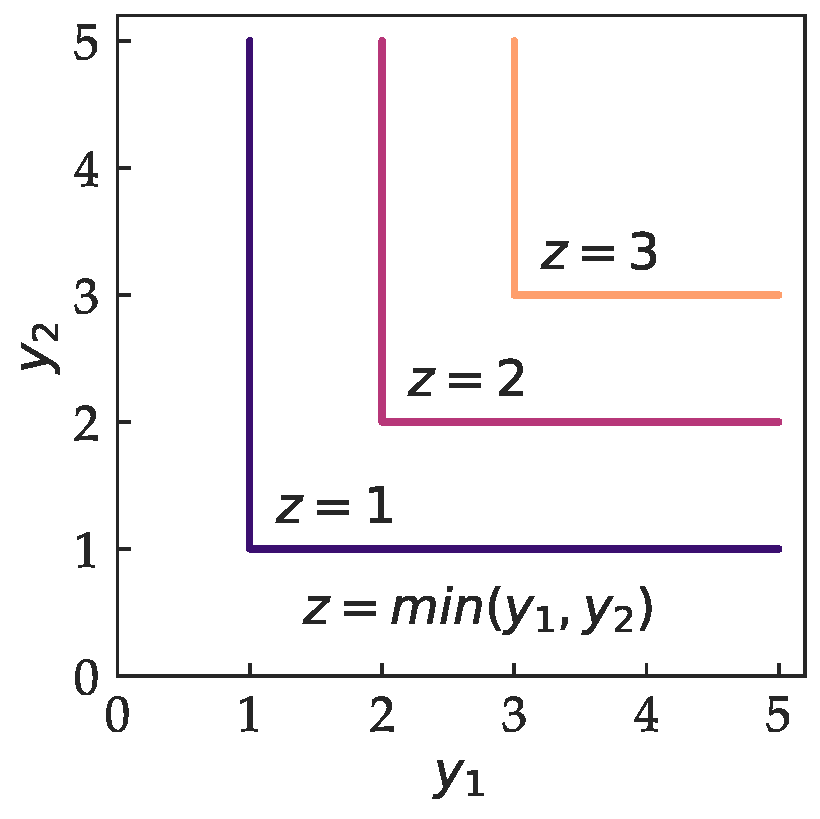
\includegraphics[width=\textwidth, height=\textwidth]{Figures/Essential.pdf}
    \end{minipage}
    \\ 
    %\begin{minipage}[t]{5cm}
    \vspace{-5pt}
    \uline{Interactive Essential:} In interactive essential interaction, we get diminishing return (instead of zero return) for a single factor: $z = y_1y_2$. If each factor is consumed using power basis function, i.e., $y_i = ax^\lambda_i$, it captures Cobb-Douglas production function.
    %\end{minipage} 
    &
    \begin{minipage}{.17\textwidth}
      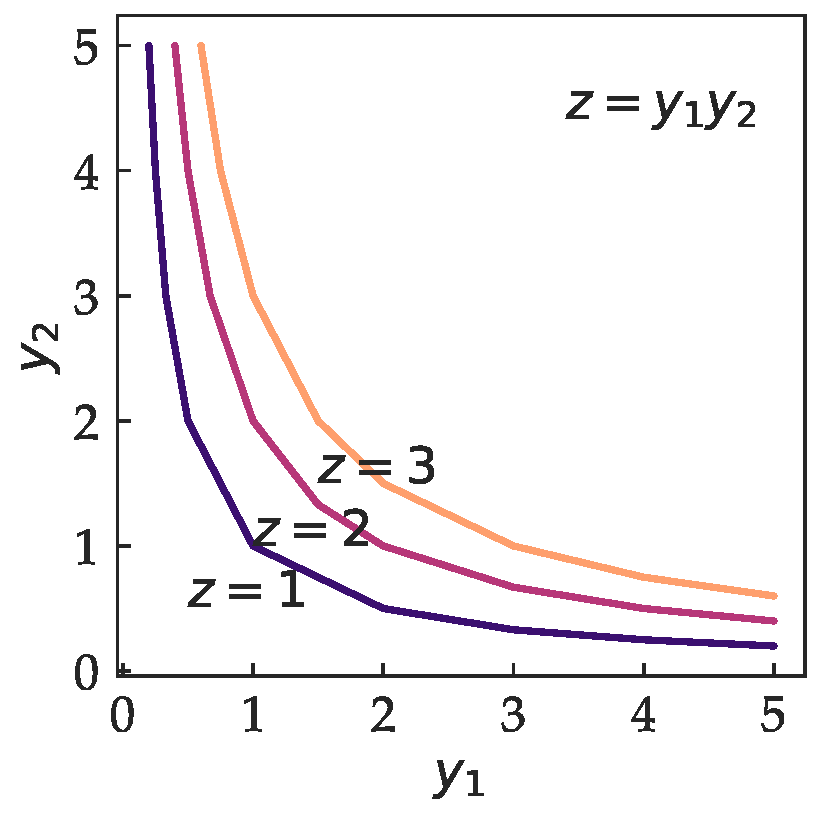
\includegraphics[width=\textwidth, height=.975\textwidth]{Figures/Interactive_Essential.pdf}
    \end{minipage}
    \\
    %\begin{minipage}[t]{5cm}
    \vspace{-5pt}
    \uline{Antagonistic:} For antagonistic factors, content generation is determined solely by the availability of the factor which yields the largest return: $z = max(y_1, y_2)$. This interaction implies that the production process has maximum possible efficiency. 
    %\end{minipage} 
    &
    \begin{minipage}{.17\textwidth}
      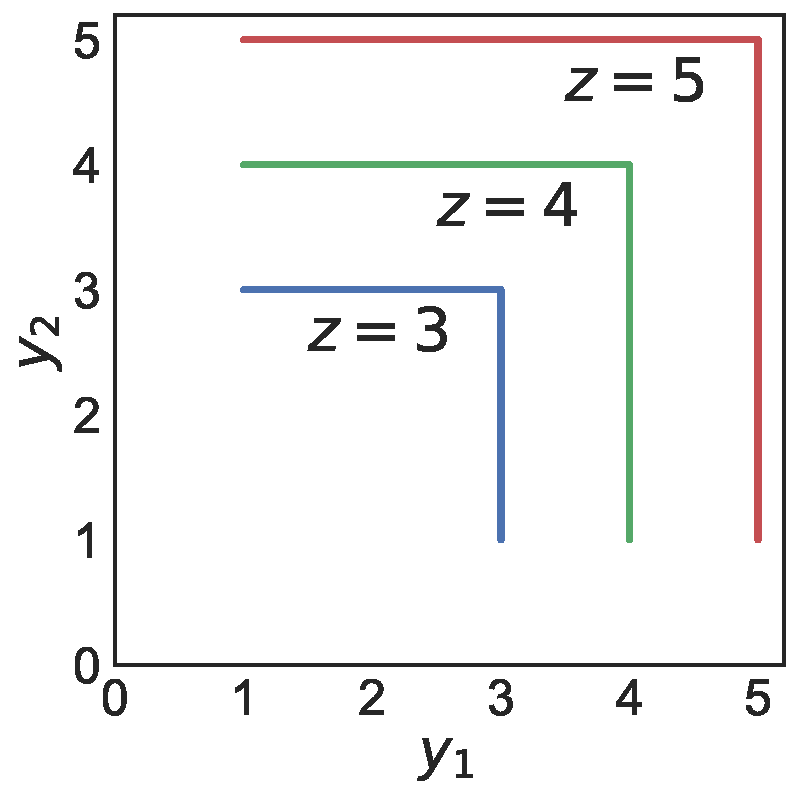
\includegraphics[width=\textwidth, height=.975\textwidth]{Figures/Antagonistic.pdf}
    \end{minipage}
    \\
    %\begin{minipage}[t]{5cm}
    \vspace{-5pt}
    \uline{Substitutable:} Factors that can each support production on their own are substitutable relative to each other: $z = w_1y_1 + w_2y_2$. This implies that there exists some equivalence between the two factors. This is similar to the general additive models.
    %\end{minipage} 
    &
    \begin{minipage}{.17\textwidth}
      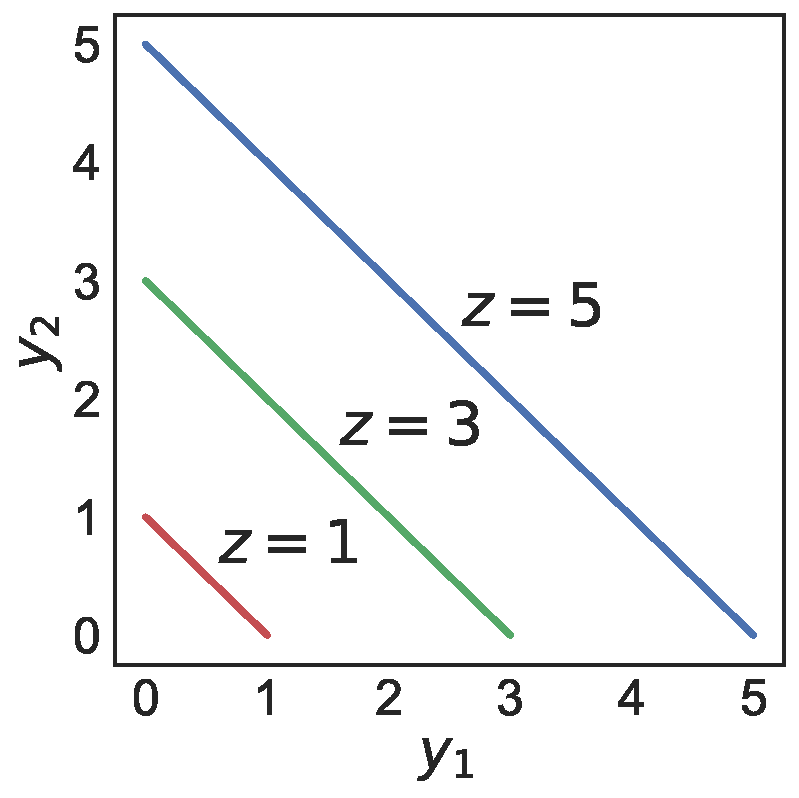
\includegraphics[width=\textwidth, height=.975\textwidth]{Figures/Substitutable.pdf}
    \end{minipage}
    \\
%    \hline
  \end{tabular}
  \vspace{-\baselineskip}
%  \caption{Pairwise interaction between factors}
  \label{tab:interaction}
\end{table}

\textbf{User to Roles.} 
We predict the number of askers, answerers, and commenters from the number of users. \textcolor{blue}{Yet to add details. Figure: LV plots to show the r-squared distribution for regression.}




\section{Dataset} 
We collected the latest release (September, 2017) of Stack Exchange dataset. This snapshot is a complete archive of all activities in all Stack Exchange. 

There are 170 sites in our collected dataset. For the purpose of empirical analysis, we only consider the sites that have been active for at least 12 months beyond the ramp up period (site created, but few or no activity). There are 157 such sites. The age of these sites vary from 14 months to 111 months, number of user from 1072 to 547175, number of posts (questions and answers) from 1600 to 1985869. In addition, the sites have small overlaps in terms of user base, ranging from 0.1\% to 12\%. Therefore, we can reasonably argue that the underlying markets are independent. 

In Figure~\ref{fig:dataset} we present letter value plots to show the distribution of number of users, number of posts, and age for the Stack Exchange markets. Letter value plots include detailed information about the tails of the distribution, which is appropriate for large dataset such as ours. 


\iffalse
\begin{wrapfigure}{R}{0.2\textwidth}
\centering
\vspace{-\baselineskip}
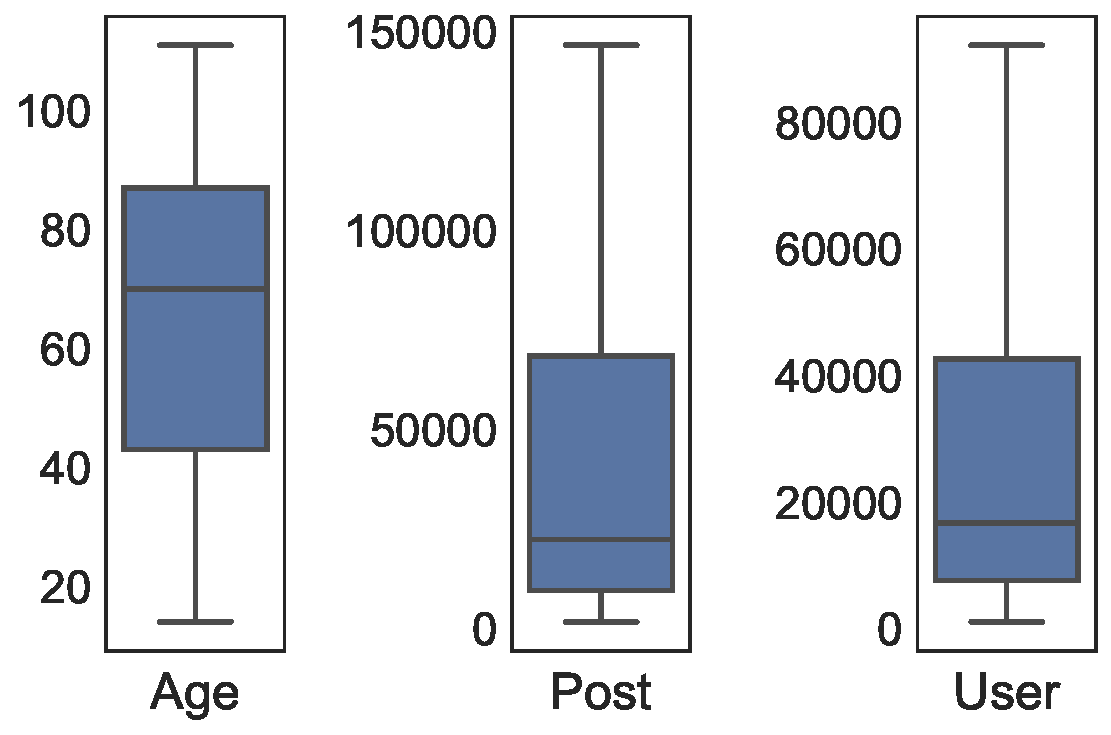
\includegraphics[width=0.2\textwidth]{Figures/Dataset_Statistics.pdf}
\caption{Site Statistics}
\vspace{-\baselineskip}
\end{wrapfigure}
\fi

\begin{figure}[hbt]
\vspace{-\baselineskip}
\centering
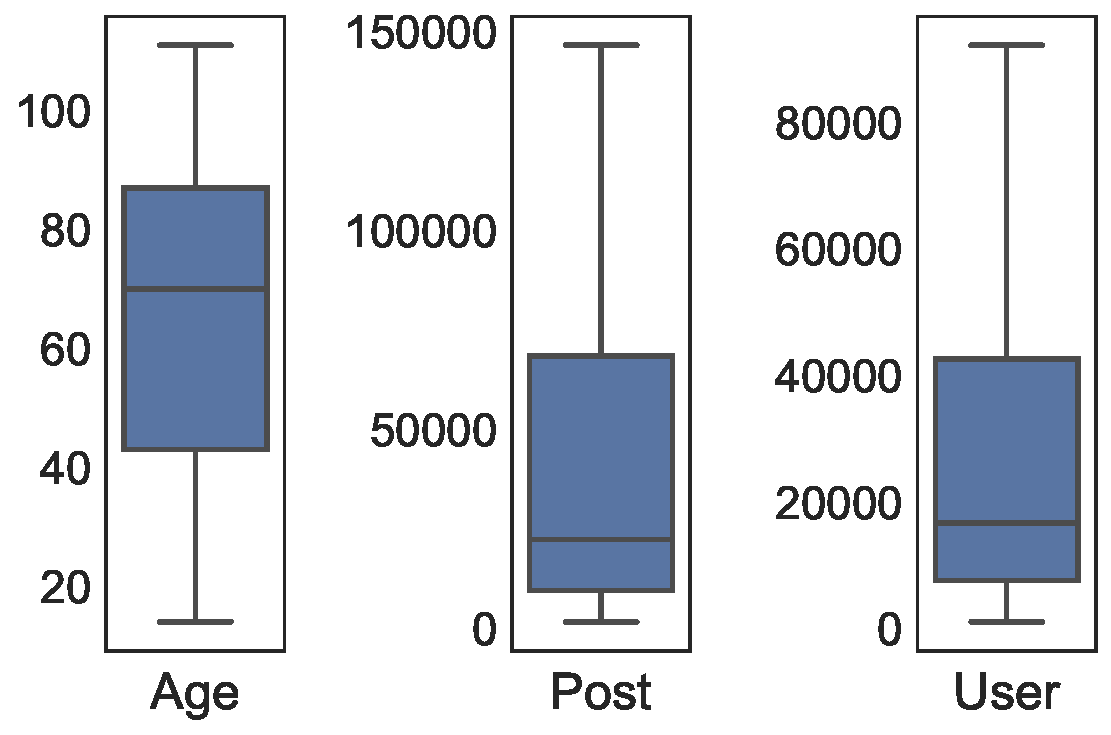
\includegraphics[scale=0.45]{Figures/Dataset_Statistics.pdf}
\vspace{-\baselineskip}
\caption{Distribution of number of users, number of posts, and age for Stack Exchange markets. The markets vary a lot in all three dimensions (users, activity, and age), as manifested by the letter value plots.}
\vspace{-\baselineskip}
\label{fig:dataset}
\end{figure}

\section{Evaluating Our Proposed Models}
In this section we examine our proposed models from three different perspectives: the accuracy of fitting content generation time series observed in our dataset (Section 6.1), the performance of predicting content volume in long and short run (Section 6.2), and the perplexity of characterizing content generation dynamics at early stage (Section 6.3).

\subsection{Model Fitting}
We fit each variant of production model for each content type to the observed time series in each Stack Exchange website. Notice that among the different variants of production models (based on the basis and aggregate functions), the models using power or exponent basis have a parsimonious set of parameters. For example, answer generation model using power/exponential basis function requires only three parameters for interactive essential interaction, and four parameters for remaining interaction types. In contrast, answer generation model using sigmoid function requires five parameters for interactive essential interaction, and six parameters for remaining interaction types. 

\textbf{Parameter Estimation.} Our parameter learning process has three sequential steps enforced by the content dependency among question, answer and comment. Therefore, we first learn the best-fit parameters for modeling question, followed by answer, followed by comment. At each step, we use the parameters learnt in earlier steps to generate input. \textcolor{blue}{Yet to add details.}

%Method ‘trf’ (Trust Region Reflective) is motivated by the process of solving a system of equations, which constitute the first-order optimality condition for a bound-constrained minimization problem as formulated in [STIR]. The algorithm iteratively solves trust-region subproblems augmented by a special diagonal quadratic term and with trust-region shape determined by the distance from the bounds and the direction of the gradient. This enhancements help to avoid making steps directly into bounds and efficiently explore the whole space of variables. To further improve convergence, the algorithm considers search directions reflected from the bounds. To obey theoretical requirements, the algorithm keeps iterates strictly feasible. With dense Jacobians trust-region subproblems are solved by an exact method very similar to the one described in [JJMore] (and implemented in MINPACK). The difference from the MINPACK implementation is that a singular value decomposition of a Jacobian matrix is done once per iteration, instead of a QR decomposition and series of Givens rotation eliminations. For large sparse Jacobians a 2-d subspace approach of solving trust-region subproblems is used [STIR], [Byrd]. The subspace is spanned by a scaled gradient and an approximate Gauss-Newton solution delivered by scipy.sparse.linalg.lsmr. When no constraints are imposed the algorithm is very similar to MINPACK and has generally comparable performance. The algorithm works quite robust in unbounded and bounded problems, thus it is chosen as a default algorithm.




%The NETTIDE for node and link together has a parsimonious set of parameters, namely, β, θ,β′, α, γ and N. Our parameter learn- ing process has two steps: to learn node equation, and to learn link equation. Given the real node growth sequence n(t), we aim to minimize the sum of the square errors: Tt=t0 (n(t) − n∗(t))2, by using the Levenberg-Marquardt algorithm (LM) [28], which is widely used to solve non-linear least squares problems [30, 13, 33]. As for link equation, given the real link and node growth sequence e(t) and n(t), and the temporal fizzling exponent θ learned by the node step, we follow the same procedure as the node step to mini- mize the sum of the square errors: Tt=t0 (e(t) − e∗(t))2.



%Our model has five parameters, namely, ↵, , , , and C. Notwithstanding the five-dimensional parameter space, the overall DAU evolution shapes allowed by the model ef- fectively has fewer degrees of freedom. The reduction in degrees of freedom is due to the relationship between  and ↵ explored in Section 3.1, the initial DAU growth di↵erences between  and  explored in Section 3.2, and the magnitude of  and  which helps dictate the DAU initial growth rate. Note that C is just a resealing parameter and does not a↵ect the shape of the DAU time series curve. Figures 4(a), 4(b), and 5(a) present three of the most common DAU evolution shapes observed in our datasets.

%The algorithm used to fit the model to the data works as follows. Let D be the set containing all datasets used in this study. We find the an optimal parameter fit to a dataset d 2 D using the Levenberg-Marquardt algorithm [36]. We use the first few years of DAUs data to train the model and the remaining h years data as holdout data to evaluate the model predictions (part of h is also user later in a model selection phase). The Levenberg-Marquardt algorithm only finds a locally optimal solution starting from an initial pa- rameter guess m0 = (↵0, 0, 0, 0, C0). Hence, the initial guess m0 may significantly influence the output of the algo- rithm. To make the algorithm fully automatic and robust we need to find a principled way to provide this initial guess using our datasets.
%We provide the initial parameter guess by feeding the Levenberg-Marquardt algorithm with other parameter ex- amples obtained in our datasets. It is reasonable to assume that the DAU time series of a given dataset d 2 D is sim- ilar to the DAU time series of some other datasets in D. If we knew the best parameter fit of a dataset with simi- lar DAU time series as d we could then use it to initialize the Levenberg-Marquardt algorithm. But as we don’t know which datasets in D\{d} (D\{d} is the set of all datasets excluding d) have similar DAU, we test all possible datasets as follows. Let LM(d,m0) be the Levenberg-Marquardt fit- ted parameters using initial guess m0. Let fd0 be the best currently known fit to dataset d0 2 D\{d}. At this stage our algorithm produces a set of candidate fitted parameters C = {LM(d,fd0) : d0 2 D\{d}}.
%Instead of selecting the best fitted parameters from C, we make our parameter selection more robust by selecting at least three fitted parameters from C. We test the quality of the fitted parameters through a model selection phase. In the model selection phase we use the first three to six months of DAU data in the holdout data (comprising of up to 10% of the total data) to assign an L2 error to the predictions of the model with each fitted parameters in C. Using these errors, together with the actual parameter val- ues, we cluster the elements of C using k-medoids clustering (using the R package pamk and the Calinski-Harabasz [8] criteria to automatically select the number of clusters k).

%We choose to use k-medoids instead of the widely used k- means because k-medoids is likely more robust to noise and outliers than k-means, in the same manner that the median of a set of measurements is more robust to noise and outliers than their mean. The output of our algorithm is then the k-medoid cluster c ✓ C that has at least three elements and the smallest average error.
%More precisely, our algorithm reports c and the medoid of c. The medoid of c is the vector of parameters that best represents all vectors of parameters in c. The above proce- dure must be bootstrapped by manually assigning parame- ter fits to the datasets. But once we automatically obtain the medoid parameter fit of d we can replace its manually initialized value with the automatic one and restart the pro- cess. The R source code of our algorithm is freely available online to be tested on other datasets2.

\textbf{Model Fitting Results.} 
Now, we present the model fitting results. \textcolor{blue}{Yet to add details.}

\begin{table}[ht]
	\vspace{-0.5\baselineskip}
	\caption{Model Fitting Results}
    \vspace{-\baselineskip}
	\label{tbl:model_fit}
	\begin{center}
	\begin{tabular}{llccc}
    \toprule
    Content & Interaction Type & RMSE & NRMSE & EVS\\
    \midrule
    Question & NA & 25.742 & 0.086 & 0.791\\
    \midrule
    \multirow{4}{*}{Answer} & Essential & 70.307 & 0.092 & 0.789\\
    & Interactive Essential & 64.624 & 0.083 & 0.825\\
    & Antagonistic & 72.765 & 0.094 &  0.778\\
    & Substitutable & 68.900 & 0.089 & 0.805\\
    \midrule
    \multirow{4}{*}{Comment} & Essential & 146.644 & 0.084 & 0.833\\
    & Interactive Essential & 137.228 & 0.081 & 0.845\\
    & Antagonistic & 155.969 & 0.088 &  0.818\\
    & Substitutable & 155.433 & 0.089 & 0.820\\
    \bottomrule
	\end{tabular}
	\end{center}
    \vspace{-\baselineskip}
\end{table}
 

%We evaluate the overall fitting accuracy using Normalized Root Mean Square Error (NRMSE). Given two series, for example the observed time series of answers $N_a(t)$
%real node growth sequence n(t) and the corresponding sequence
%(n(t)−n∗(t))2 n∗(t) given by our model, NRMSE= T t=1
%a special case when T = 1, NRMSE degenerates to Absolute Per-
%centage Error (APE(x, x∗ ) = |x−x∗ | ). NRMSE is consistent with
%x
%the objective function of the LM algorithm in the sense of L2 nor- m. And also it can be compared between datasets with different scales. We also compare the performance by other standard metric, namely Mean Absolute Percentage Error (MAPE). We get consis- tent conclusion and thus we do not report it for brevity. Table 3 shows the description of the best fitting parameters to four datasets.

\subsection{Forecasting Content Generation} 
We apply the best-fit production models to predict content volume in long and short run. \textcolor{blue}{Yet to add details.}

\begin{table}[ht]
	\vspace{-0.5\baselineskip}
	\caption{Model Prediction Results}
    \vspace{-\baselineskip}
	\label{tbl:model_prediction}
	\begin{center}
	\begin{tabular}{llccc}
    \toprule
    Content & RMSE & NRMSE\\
    \midrule
    Question & 35.412 & 0.291\\
    Answer & 113.341 & 0.117\\
    Comment & 195.234 & 0.274\\
    \bottomrule
	\end{tabular}
	\end{center}
    \vspace{-\baselineskip}
\end{table}

We study the effectiveness of our models under different time granularity, e.g., day, week, month, quarter. \textcolor{blue}{Figure: Yet to add details. Table: Present prediction accuracy for different time granularity (bar chart)}

\subsection{Parameter Estimation for New Websites} 
We use parameters learnt from old Stack Exchange websites as priors for new Stack Exchange websites. \textcolor{blue}{Yet to add details. Table: Present error in parameter estimation.}





\section{Characterizing Knowledge Markets}
In this section we characterize the knowledge markets in Stack Exchange---explaining the best-fit models and their foundations (Section 7.1), revealing two key distributions that control the markets (Section 7.2), and uncovering the stable core that maintains market equilibrium (Section 7.3).

\subsection{Model Interpretation} 
First, we explain the best-fit models found in Section 6.1. We observe that content generation in Stack Exchange markets are best modeled through the combination of power basis and interactive essential interaction. In addition, we found that the best-fit exponents ($\lambda$ parameter in basis $g(x) = ax^\lambda$, where $x$ is a factor) of these models lie between 0 and 1 (inclusive), for all factors of all content types, for all Stack Exchange. 

A model that uses power basis (where exponents lie between 0 and 1) and interactive essential interaction is known as the Cobb-Douglas production function~\cite{wiki}. In its most standard form for production of a single output $z$ with two inputs $x_1$ and $x_2$, the function is: 
$$z = ax_1^{\lambda_1}x_2^{\lambda_2}.$$
Here, coefficient $a$ represents the \emph{total factor productivity}---the portion of output not explained by the amount of inputs used in production~\cite{wiki}. As such, its level is determined by how efficiently the inputs are utilized in production. The exponents $\lambda$s represent the \emph{output elasticity} of the inputs---the percentage change in output that results from the percentage change in a particular input~\cite{wiki}. 

The Cobb-Douglas function provides intuitive explanation for content generation in Stack Exchange markets. In particular, the explanation stands on three phenomena or principles: constant elasticity, diminishing returns, and returns to scale.

\textbf{Constant Elasticity.} In Stack Exchange markets, factors such as user participation and content dependency have \emph{constant elasticity}---percentage increase in any of these inputs will have constant percentage increase in output~\cite{wiki}, as claimed by the corresponding exponents in the model. For example, in \texttt{academia} ($N_A = 6.93N_q^{0.18}U_a^{0.65}$), 1\% increase in number of answerers ($U_a$) leads to 0.65\% increase in number of answers ($N_a$). 

\textbf{Diminishing Returns.} For a particular factor, when the exponent is less than 1, we observe \emph{diminishing returns}---decrease in the marginal (incremental) output as an input is incrementally increased, while the other inputs are kept constant~\cite{wiki}. This \lq law of diminishing returns\rq\ has many interesting implications for the Stack Exchange markets, including the diminishing benefit of having a new participant in a market. For example, in \texttt{academia}, if the number of answerers is 100, then the marginal contribution of a new answerer is $c(101^{0.65} - 100^{0.65}) = 0.129c$, where $c$ is a constant; in contrast, if the number of answerers is 110, then the marginal contribution of a new answerer is $c(111^{0.65} - 110^{0.65}) = 0.125c$. Thus, for answer generation in \texttt{academia}, including a participant when the number of participants (system size) is 110 is likely to be less beneficial compared to including a participant when the system size is 100.

\textbf{Returns to scale.} The knowledge markets in Stack Exchange vary in terms of scale efficiency, as manifested by their \emph{returns to scale}---the increase in output resulting from a proportionate increase in all inputs~\cite{wiki}. If a market has high returns to scale, then greater efficiency is obtained as the market moves from small- to large-scale operations. For example, in \texttt{academia}, for answer generation, the returns to scale is $0.18+0.65=0.83<1$. The market becomes less efficient as answer generation is expanded, requiring more questions and answerers to increase the number of answers by same amount. 

\subsection{Two Key Distributions} 
Next, we discuss two key distributions that control content generation in knowledge markets, namely participant activity and subject POV (perspective). These two distributions induce the three phenomena reported in section 7.1. 

\textbf{Participant Activity.} The distribution of participant activities implicitly drives a market's return in terms of user participation, as manifested by the corresponding exponent. For example, in a hypothetical knowledge market where each answerer contributes equally, the answer generation model should be $N_a = AN_q^{\lambda_1}U_a^{1.0}$. In reality, the distribution of participant activities is a size dependent distribution controlled by the number of participants (system size). As the system size increases, most participants contribute to the head of the distribution (few activities), whereas very few join the tail (many activities). 

We systematically reveal the size dependent distribution for participant activities in three steps. First, we empirically fit power-law distribution to the activities of participants in a month, for each month, for each Stack Exchange. We follow the standard procedure to fit a power-law distribution. We observe that power-law well describe the monthly activity distributions. Second, we plot the exponents of power-law against the number of participants for all observed months in a Stack Exchange, for each Stack Exchange. We observe that for most Stack Exchange power-law exponent decreases as the system size increases. Third, we apply linear regression to reveal the relationship between power-law exponents and system size. We observe that in general power-law exponents are negatively correlated with system size. This negative correlation is strongly visible in big knowledge markets that have at least 500 monthly participants in each month.

\begin{figure}[hbt]
\vspace{-0.5\baselineskip}
\centering
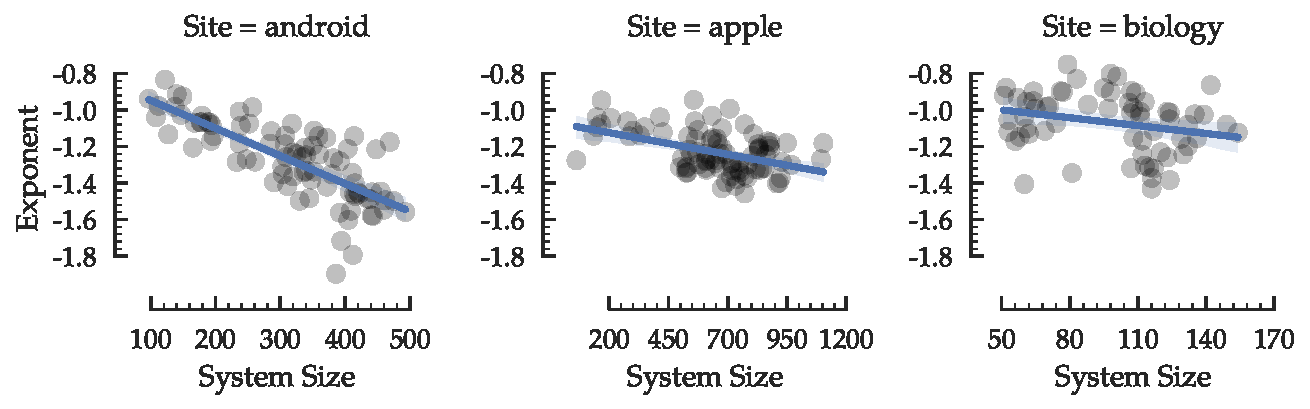
\includegraphics[scale=0.38]{Figures/Size_Dependent_Distribution.pdf}
\vspace{-2\baselineskip}
\caption{The visibility of size dependent distribution in \texttt{android} (strong), \texttt{apple} (moderate), and \texttt{biology} (weak). In most markets, the power-law exponent decreases with system size (similar to academia). In other markets, there exists a non-zero correlation between system size and power-law exponent.}
\vspace{-\baselineskip}
\label{fig:sdd}
\end{figure}

In Figure~\ref{fig:sdd} we present empirical evidence of size dependent distribution for answer generation in three markets: \texttt{android}, \texttt{apple}, and \texttt{biology}. We choose these examples to cover three possible visibility of size dependent distribution, as manifested by the correlation between 
power law exponent and system size---strong correlation ($|r^2|>0.5$), moderate correlation($0.3<|r^2|<0.5$), weak correlation ($|r^2|<0.3$).

\textbf{Subject POV.} The distribution of subject POV implicitly drives a market's return in terms of content dependency, as manifested by the corresponding exponent. Subject POV refers to the number of distinct perspectives on a particular content (primarily question) that imposes a conceptual limit to the number of dependent contents (answers). For example, an open-ended question such as \lq What's your favorite book?\rq\ has many possible answers, whereas a close-ended question such as \lq What's the solution for 3x+5 = 2?\rq\ has a single correct answer. In reality, most questions are neither completely open-ended nor completely closed; however, from an answerer's perspective, there's a diminishing utility in answering a question that already has an answer. This diminishing utility varies from question to question---questions asking for recommendations attract many answers, whereas questions seeking factual information attract few answers. 

\subsection{Uncovering the Stable Core} 
Now, we discuss about the core user community that assist maintaining the Cobb-Douglas models in a knowledge market. The Cobb-Douglas models indicate the presence of dynamic equilibria where the increase or decrease in user community does not affect the models. To this end, we assert that there is a stable user community in each knowledge markets who contribute a large fraction of contents; whereas the remaining users are unstable and contribute a small fraction. This is particularly applicable for contents that require more effort, e.g, answers and comments. 

We reveal the presence of core user community by summarizing the age of users with different levels of contribution for all Stack Exchange. First, we categorize all users in Stack Exchange using quartiles based on average number of contributions per month. Then, for each user in each market, we compute normalized age by dividing the user's age (number of active months) with the maximum possible age in the market. Next, we summarize the normalized age of users with same levels of contribution for all markets using letter value plots. This allows us to observe the global distribution of normalized age for users with varying levels of monthly contribution. We present these distributions in Figure~\ref{fig:age_vs_contribution}. We observe that there is a clear gap between the distribution of age of users for any two levels of contribution---users in 4th quartile (who contribute a lot) have highest normalized age, followed by 3rd and 2nd quartile. 

\begin{figure}[hbt]
\centering
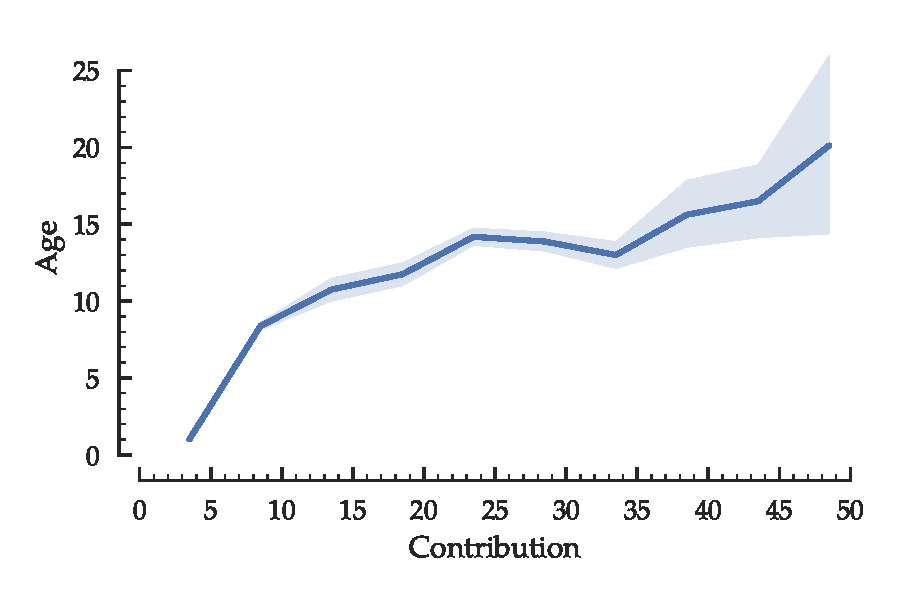
\includegraphics[scale=0.5]{Figures/Age_vs_Contribution.pdf}
\caption{The global distribution of age for users with varying levels of monthly contribution. The users who contribute most to a market on a monthly basis, also contribute for many months as manifested by the age}
\label{fig:age_vs_contribution}
\end{figure}



\section{Failures at Scale}
In this section we discuss how and why knowledge markets may fail at scale. We first empirically examine diseconomies of scale (Section 8.1), then analyze the effects of scale on market health (Section 8.2), and finally study market stability under user perturbation (Section 8.3).

\subsection{Diseconomies of Scale}
First, we examine disceconomies of scale---the ratio of answers to questions declining with the increase in number of users. The opposite of diseconomies is economies---the ratio of answers to questions increasing with the increase in number of users. The concept of diseconomies is important because the decrease in answer to question ratio implies the increase in the gap between market supply (answer) and demand (question). In fact, if the ratio falls below 1.0, the gap becomes critical---guaranteeing there will be some questions with no answers. We observe disceconomies of scale in most Stack Exchange markets.

Figure~\ref{fig:diseconomy} shows three examples of diseconomies and economies (the reverse of diseconomies): \texttt{cstheory}, \texttt{puzzling} and \texttt{superuser}. Among the three markets, \texttt{superuser} shows strong diseconomies of scale---if the number of users increases by 100\%, the answer to question ratio declines by a factor of x.x. The other two markets are counter examples, where \texttt{cstheory} shows strong economies of scale---if the number of users increases by 100\%, the answer to question ratio increases by a factor of x.x; and \texttt{puzzling} shows weak economies of scale---if the number of users increases by 100\%, the answer to question ratio increases by a factor of x.x. Note that most markets, especially the ones with 500+ monthly active participants, exhibit diseconomies of scale similar to \texttt{superuser}. The markets that exhibit economies of scale are rare; we found four such markets in Stack Exchange: \texttt{cstheory}, \texttt{expressionengine}, \texttt{softwareengineering}, \texttt{hardwarerecs}.

\begin{figure}[hbt]
\vspace{-0.5\baselineskip}
\centering
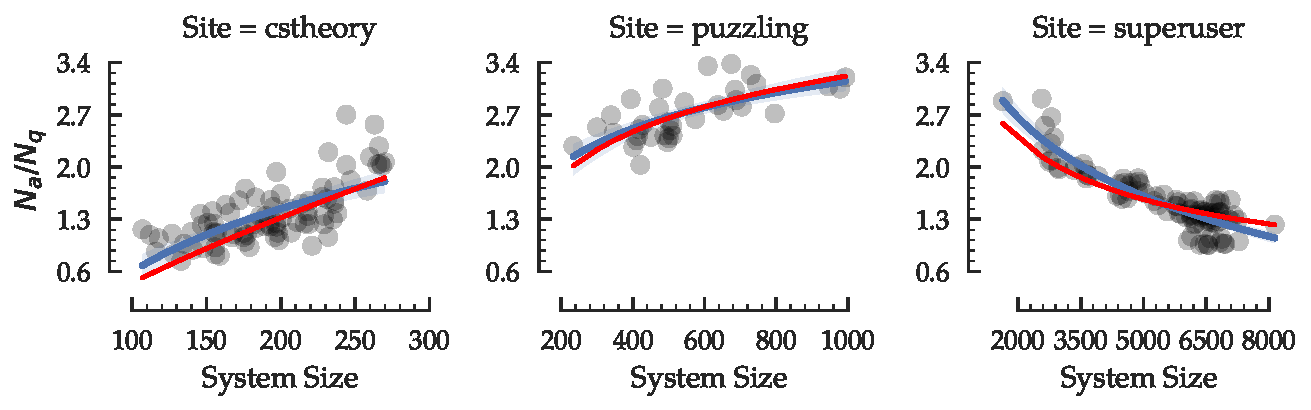
\includegraphics[scale=0.38]{Figures/Size_vs_Diseconomy.pdf}
\vspace{-2\baselineskip}
\caption{Economies and disecnomies of scale: \texttt{cstheory} (strong economies), \texttt{puzzling} (weak economies) and \texttt{superuser} (strong diseconomies). Most markets exhibit diseconomies of scale similar to \texttt{superuser}.}
\vspace{-\baselineskip}
\label{fig:diseconomy}
\end{figure}

The Cobb-Douglas curves well fit the empirical trends of economies and diseconomies. We derive these curves by dividing the answer models by the corresponding question models. We get similar curves via log regression as shown in Figure~\ref{fig:diseconomy}. Between the two model types, the Cobb-Douglas models provide better explanation.

The Cobb-Douglas models well explain the economies and disceconomies of scale. Based on the models, the primary cause of disceconomies is the difference between the diminishing returns of questions and answers for users. In other words, in most market, for user input, the marginal question output is higher compared to marginal answer output, i.e., an average user is likely to ask more questions and provide few answers. This causes the ratio of answers to questions to decline with the increase in number of users.

\subsection{Analyzing Health}
Next, we examine the disadvantage of scale through three health metrics: $H_1.$ percentage of answered questions (questions with at least one answer), $H_2.$ percentage of questions with accepted answer, and $H_3$. average number of upvotes per content. The first two metrics capture the utility received by askers, whereas the third metric captures the utility received by any active user. The decline in answer to question ratio may cause decline in the first two health metrics. In fact, if the ratio falls below 1.0, it guarantees the decline of these metrics. Figure x shows the disadvantage of scale through health metrics for three markets: academia, android and tex. We observe that all three health metrics decline at scale. \textcolor{blue}{Figure: Plot to show the decline of health metrics at scale.}

We cluster the markets based on model parameters and examine their health. In particular, we use kmeans clustering with silhouette analysis to determine two clusters. Figure x shows the clusters in a 3d space, reduced via Isomap reduction. Figure y shows the health summary for the two clusters. There exists a clear gap between the health of the two clusters. The first group is somewhat more robust to scale, whereas the second group is vulnerable at scale.

\begin{figure}[hbt]
\vspace{-0.5\baselineskip}
\centering
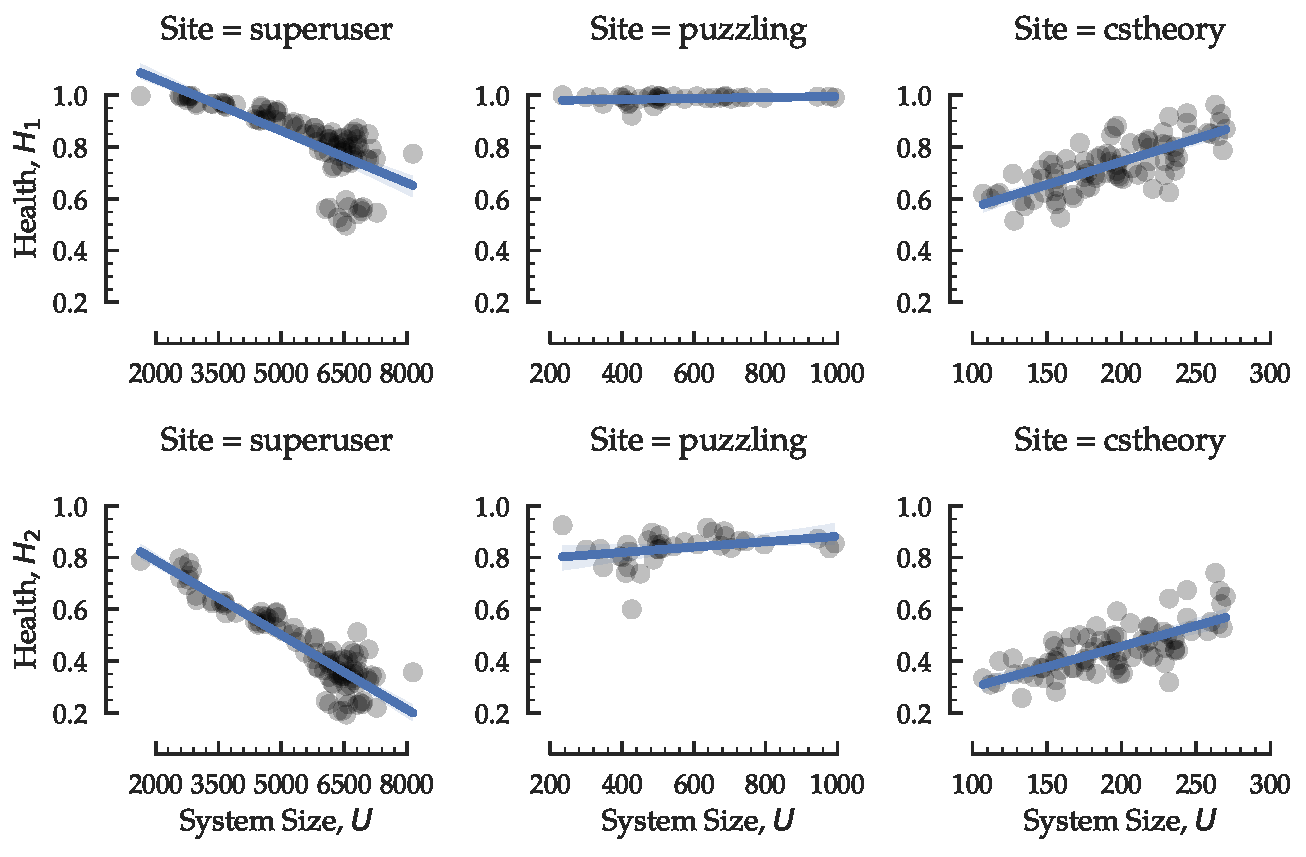
\includegraphics[scale=0.38]{Figures/Size_vs_Health.pdf}
\vspace{-2\baselineskip}
\caption{Long caption}
\vspace{-\baselineskip}
\label{fig:health}
\end{figure}

\subsection{Effects on Stability}
Now, we study market stability under user perturbation. We concentrate on how many users
As the stability of knowledge markets depend on user participation, we investigate the effect of scale on stability. \textcolor{blue}{Yet to add details. Figure: Plot to show stability as a function of economic parameters/size/etc.}

\begin{figure}[hbt]
\vspace{-0.5\baselineskip}
\centering
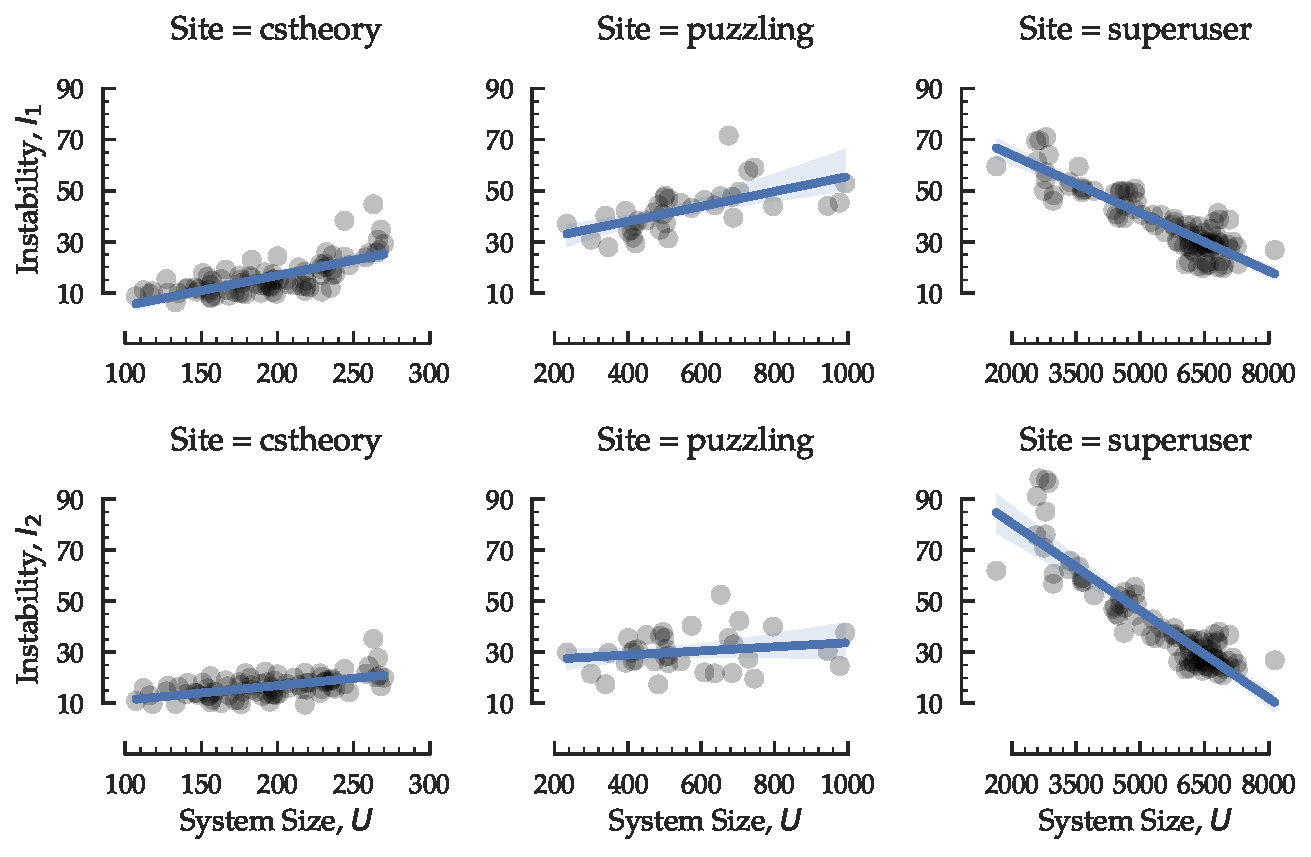
\includegraphics[scale=0.38]{Figures/Size_vs_Instability.pdf}
\vspace{-2\baselineskip}
\caption{Long caption}
\vspace{-\baselineskip}
\label{fig:stability}
\end{figure}



\section{Discussion}
In this section we discuss the analytical findings of our model (Section 8.1) along with a couple of complementary and alternative models (Section 8.2).

\subsection{Analytical Findings}
We present several analytical findings that have implications for different aspects of knowledge markets. \textcolor{blue}{Yet to add details.}

\subsection{Limitation}
\textcolor{blue}{Yet to add details.}

\iffalse
\subsection{Complementary and Alternative Models}
We consider several alternative models to comprehend the content generation dynamics in knowledge markets. Our first attempt is to model user content generation as \lq self-exciting\rq\ point process. In this attempt, we design and implement several variants of Hawkes process. Our second attempt is to model user content generation using \lq stage-structured\rq\ projection matrix. In this attempt, we build variants of Leftkovitch matrix. 

\textbf{Hawkes Process.} The Hawkes process is a mathematical model for self-exciting processes that models a sequence of arrivals of some event over time, e.g., natural disasters, gang violence, trade orders.  Each arrival excites the process in the sense that the chance of a subsequent arrival is increased for some time period after the initial arrival. 

Content generation in Stack Exchange websites can be conceptualized as Hawkes process with multiple event types. Here, arrival of certain type of event (e.g., questions) excites the arrival of other types of event (e.g., answers, comments). 

A univariate Hawkes process is defined to be a self-exciting temporal point process $N$ whose conditional intensity function $\lambda = \lambda(t)$ is defined to be

 $$\lambda(t) = \mu(t)+\sum_{i:\tau_i<t}g(t-\tau_i),$$
 
where $\mu(t)$ is the background rate of the process  $N$, where $\tau_i$ are the points/events in time occurring prior to time t, and where $g$ is a function which governs the clustering density of N. 

The multi-dimensional Hawkes process is defined by a $U$-dimensional point process $N_t^u, u =1, . . . , U$, with the conditional intensity for the $u$-th dimension expressed as follows:
$$\lambda_u(t) = \mu_u + \sum_{i:\tau_i<t} g_{uu_i}(t-\tau_i),$$

where $\mu_u \ge 0$ is the base intensity for the $u$-th Hawkes process. The kernel $g_{uu^\prime}(t) \ge 0$ captures the mutually exciting property between the $u$-th and $u^\prime$-th dimension. Intuitively, it captures the dynamics of influence of events occurred in the $u^\prime$-th dimension to the $u$-th dimension. Larger value of $g_{uu^\prime}(t)$  indicates that events in $u^\prime$-th dimension are more likely to trigger a event in the $u$-th dimension after a time interval $t$.

\textbf{Leftkovitch Matrix.} \textcolor{red}{A brief description of the Leftkovitch Matrix based models.}
\fi



\section{Conclusion}

%\documentclass[sigconf]{acmart}

\usepackage{booktabs} % For formal tables
% My packages
\usepackage{tikz}
\usetikzlibrary{bayesnet}
\usepackage[normalem]{ulem}
\usepackage{wrapfig}
\usepackage{xcolor}
\usepackage{array}
\newcommand{\hs}[1]{\textcolor{red}{Hari: #1}}

% Copyright
%\setcopyright{none}
%\setcopyright{acmcopyright}
%\setcopyright{acmlicensed}
%\setcopyright{rightsretained}
%\setcopyright{usgov}
%\setcopyright{usgovmixed}
%\setcopyright{cagov}
%\setcopyright{cagovmixed}


% DOI
%\acmDOI{10.475/123_4}

% ISBN
%\acmISBN{123-4567-24-567/08/06}

%Conference
\iffalse
\acmConference[WOODSTOCK'97]{ACM Woodstock conference}{July 1997}{El
  Paso, Texas USA}
\acmYear{1997}
\fi

%\copyrightyear{2016}

%\acmPrice{15.00}


\begin{document}
\title[Too Big to Succeed]{Too Big to Succeed: Understanding Successes and Failures at Scale in Knowledge Markets}

\iffalse
\titlenote{Produces the permission block, and
  copyright information}
\subtitle{Extended Abstract}
\subtitlenote{The full version of the author's guide is available as
  \texttt{acmart.pdf} document}
\fi

\author{Anonymous Author}
\affiliation{%
  \institution{Anonymous Institution}
  \city{City, Country}
}
\email{e-mail}

\iffalse
\author{Ben Trovato}
\authornote{Dr.~Trovato insisted his name be first.}
\orcid{1234-5678-9012}
\affiliation{%
  \institution{Institute for Clarity in Documentation}
  \streetaddress{P.O. Box 1212}
  \city{Dublin}
  \state{Ohio}
  \postcode{43017-6221}
}
\email{trovato@corporation.com}

\author{G.K.M. Tobin}
\authornote{The secretary disavows any knowledge of this author's actions.}
\affiliation{%
  \institution{Institute for Clarity in Documentation}
  \streetaddress{P.O. Box 1212}
  \city{Dublin}
  \state{Ohio}
  \postcode{43017-6221}
}
\email{webmaster@marysville-ohio.com}

\author{Lars Th{\o}rv{\"a}ld}
\authornote{This author is the
  one who did all the really hard work.}
\affiliation{%
  \institution{The Th{\o}rv{\"a}ld Group}
  \streetaddress{1 Th{\o}rv{\"a}ld Circle}
  \city{Hekla}
  \country{Iceland}}
\email{larst@affiliation.org}

\author{Lawrence P. Leipuner}
\affiliation{
  \institution{Brookhaven Laboratories}
  \streetaddress{P.O. Box 5000}}
\email{lleipuner@researchlabs.org}

\author{Sean Fogarty}
\affiliation{%
  \institution{NASA Ames Research Center}
  \city{Moffett Field}
  \state{California}
  \postcode{94035}}
\email{fogartys@amesres.org}

\author{Charles Palmer}
\affiliation{%
  \institution{Palmer Research Laboratories}
  \streetaddress{8600 Datapoint Drive}
  \city{San Antonio}
  \state{Texas}
  \postcode{78229}}
\email{cpalmer@prl.com}

\author{John Smith}
\affiliation{\institution{The Th{\o}rv{\"a}ld Group}}
\email{jsmith@affiliation.org}

\author{Julius P.~Kumquat}
\affiliation{\institution{The Kumquat Consortium}}
\email{jpkumquat@consortium.net}
\fi

% The default list of authors is too long for headers}
%\renewcommand{\shortauthors}{B. Trovato et al.}

\iffalse
\begin{abstract}
This paper provides a sample of a \LaTeX\ document which conforms,
somewhat loosely, to the formatting guidelines for
ACM SIG Proceedings.\footnote{This is an abstract footnote}
\end{abstract}

%
% The code below should be generated by the tool at
% http://dl.acm.org/ccs.cfm
% Please copy and paste the code instead of the example below.
%
\begin{CCSXML}
<ccs2012>
 <concept>
  <concept_id>10010520.10010553.10010562</concept_id>
  <concept_desc>Computer systems organization~Embedded systems</concept_desc>
  <concept_significance>500</concept_significance>
 </concept>
 <concept>
  <concept_id>10010520.10010575.10010755</concept_id>
  <concept_desc>Computer systems organization~Redundancy</concept_desc>
  <concept_significance>300</concept_significance>
 </concept>
 <concept>
  <concept_id>10010520.10010553.10010554</concept_id>
  <concept_desc>Computer systems organization~Robotics</concept_desc>
  <concept_significance>100</concept_significance>
 </concept>
 <concept>
  <concept_id>10003033.10003083.10003095</concept_id>
  <concept_desc>Networks~Network reliability</concept_desc>
  <concept_significance>100</concept_significance>
 </concept>
</ccs2012>
\end{CCSXML}

\ccsdesc[500]{Computer systems organization~Embedded systems}
\ccsdesc[300]{Computer systems organization~Redundancy}
\ccsdesc{Computer systems organization~Robotics}
\ccsdesc[100]{Networks~Network reliability}


\keywords{ACM proceedings, \LaTeX, text tagging}
\fi


\maketitle


%\documentclass[sigconf]{acmart}

\usepackage{booktabs} % For formal tables
% My packages
\usepackage{tikz}
\usetikzlibrary{bayesnet}
\usepackage[normalem]{ulem}
\usepackage{wrapfig}
\usepackage{xcolor}
\usepackage{array}
\newcommand{\hs}[1]{\textcolor{red}{Hari: #1}}

% Copyright
%\setcopyright{none}
%\setcopyright{acmcopyright}
%\setcopyright{acmlicensed}
%\setcopyright{rightsretained}
%\setcopyright{usgov}
%\setcopyright{usgovmixed}
%\setcopyright{cagov}
%\setcopyright{cagovmixed}


% DOI
%\acmDOI{10.475/123_4}

% ISBN
%\acmISBN{123-4567-24-567/08/06}

%Conference
\iffalse
\acmConference[WOODSTOCK'97]{ACM Woodstock conference}{July 1997}{El
  Paso, Texas USA}
\acmYear{1997}
\fi

%\copyrightyear{2016}

%\acmPrice{15.00}


\begin{document}
\title[Too Big to Succeed]{Too Big to Succeed: Understanding Successes and Failures at Scale in Knowledge Markets}

\iffalse
\titlenote{Produces the permission block, and
  copyright information}
\subtitle{Extended Abstract}
\subtitlenote{The full version of the author's guide is available as
  \texttt{acmart.pdf} document}
\fi

\author{Anonymous Author}
\affiliation{%
  \institution{Anonymous Institution}
  \city{City, Country}
}
\email{e-mail}

\iffalse
\author{Ben Trovato}
\authornote{Dr.~Trovato insisted his name be first.}
\orcid{1234-5678-9012}
\affiliation{%
  \institution{Institute for Clarity in Documentation}
  \streetaddress{P.O. Box 1212}
  \city{Dublin}
  \state{Ohio}
  \postcode{43017-6221}
}
\email{trovato@corporation.com}

\author{G.K.M. Tobin}
\authornote{The secretary disavows any knowledge of this author's actions.}
\affiliation{%
  \institution{Institute for Clarity in Documentation}
  \streetaddress{P.O. Box 1212}
  \city{Dublin}
  \state{Ohio}
  \postcode{43017-6221}
}
\email{webmaster@marysville-ohio.com}

\author{Lars Th{\o}rv{\"a}ld}
\authornote{This author is the
  one who did all the really hard work.}
\affiliation{%
  \institution{The Th{\o}rv{\"a}ld Group}
  \streetaddress{1 Th{\o}rv{\"a}ld Circle}
  \city{Hekla}
  \country{Iceland}}
\email{larst@affiliation.org}

\author{Lawrence P. Leipuner}
\affiliation{
  \institution{Brookhaven Laboratories}
  \streetaddress{P.O. Box 5000}}
\email{lleipuner@researchlabs.org}

\author{Sean Fogarty}
\affiliation{%
  \institution{NASA Ames Research Center}
  \city{Moffett Field}
  \state{California}
  \postcode{94035}}
\email{fogartys@amesres.org}

\author{Charles Palmer}
\affiliation{%
  \institution{Palmer Research Laboratories}
  \streetaddress{8600 Datapoint Drive}
  \city{San Antonio}
  \state{Texas}
  \postcode{78229}}
\email{cpalmer@prl.com}

\author{John Smith}
\affiliation{\institution{The Th{\o}rv{\"a}ld Group}}
\email{jsmith@affiliation.org}

\author{Julius P.~Kumquat}
\affiliation{\institution{The Kumquat Consortium}}
\email{jpkumquat@consortium.net}
\fi

% The default list of authors is too long for headers}
%\renewcommand{\shortauthors}{B. Trovato et al.}

\iffalse
\begin{abstract}
This paper provides a sample of a \LaTeX\ document which conforms,
somewhat loosely, to the formatting guidelines for
ACM SIG Proceedings.\footnote{This is an abstract footnote}
\end{abstract}

%
% The code below should be generated by the tool at
% http://dl.acm.org/ccs.cfm
% Please copy and paste the code instead of the example below.
%
\begin{CCSXML}
<ccs2012>
 <concept>
  <concept_id>10010520.10010553.10010562</concept_id>
  <concept_desc>Computer systems organization~Embedded systems</concept_desc>
  <concept_significance>500</concept_significance>
 </concept>
 <concept>
  <concept_id>10010520.10010575.10010755</concept_id>
  <concept_desc>Computer systems organization~Redundancy</concept_desc>
  <concept_significance>300</concept_significance>
 </concept>
 <concept>
  <concept_id>10010520.10010553.10010554</concept_id>
  <concept_desc>Computer systems organization~Robotics</concept_desc>
  <concept_significance>100</concept_significance>
 </concept>
 <concept>
  <concept_id>10003033.10003083.10003095</concept_id>
  <concept_desc>Networks~Network reliability</concept_desc>
  <concept_significance>100</concept_significance>
 </concept>
</ccs2012>
\end{CCSXML}

\ccsdesc[500]{Computer systems organization~Embedded systems}
\ccsdesc[300]{Computer systems organization~Redundancy}
\ccsdesc{Computer systems organization~Robotics}
\ccsdesc[100]{Networks~Network reliability}


\keywords{ACM proceedings, \LaTeX, text tagging}
\fi


\maketitle


%\documentclass[sigconf]{acmart}

\usepackage{booktabs} % For formal tables
% My packages
\usepackage{tikz}
\usetikzlibrary{bayesnet}
\usepackage[normalem]{ulem}
\usepackage{wrapfig}
\usepackage{xcolor}
\usepackage{array}
\newcommand{\hs}[1]{\textcolor{red}{Hari: #1}}

% Copyright
%\setcopyright{none}
%\setcopyright{acmcopyright}
%\setcopyright{acmlicensed}
%\setcopyright{rightsretained}
%\setcopyright{usgov}
%\setcopyright{usgovmixed}
%\setcopyright{cagov}
%\setcopyright{cagovmixed}


% DOI
%\acmDOI{10.475/123_4}

% ISBN
%\acmISBN{123-4567-24-567/08/06}

%Conference
\iffalse
\acmConference[WOODSTOCK'97]{ACM Woodstock conference}{July 1997}{El
  Paso, Texas USA}
\acmYear{1997}
\fi

%\copyrightyear{2016}

%\acmPrice{15.00}


\begin{document}
\title[Too Big to Succeed]{Too Big to Succeed: Understanding Successes and Failures at Scale in Knowledge Markets}

\iffalse
\titlenote{Produces the permission block, and
  copyright information}
\subtitle{Extended Abstract}
\subtitlenote{The full version of the author's guide is available as
  \texttt{acmart.pdf} document}
\fi

\author{Anonymous Author}
\affiliation{%
  \institution{Anonymous Institution}
  \city{City, Country}
}
\email{e-mail}

\iffalse
\author{Ben Trovato}
\authornote{Dr.~Trovato insisted his name be first.}
\orcid{1234-5678-9012}
\affiliation{%
  \institution{Institute for Clarity in Documentation}
  \streetaddress{P.O. Box 1212}
  \city{Dublin}
  \state{Ohio}
  \postcode{43017-6221}
}
\email{trovato@corporation.com}

\author{G.K.M. Tobin}
\authornote{The secretary disavows any knowledge of this author's actions.}
\affiliation{%
  \institution{Institute for Clarity in Documentation}
  \streetaddress{P.O. Box 1212}
  \city{Dublin}
  \state{Ohio}
  \postcode{43017-6221}
}
\email{webmaster@marysville-ohio.com}

\author{Lars Th{\o}rv{\"a}ld}
\authornote{This author is the
  one who did all the really hard work.}
\affiliation{%
  \institution{The Th{\o}rv{\"a}ld Group}
  \streetaddress{1 Th{\o}rv{\"a}ld Circle}
  \city{Hekla}
  \country{Iceland}}
\email{larst@affiliation.org}

\author{Lawrence P. Leipuner}
\affiliation{
  \institution{Brookhaven Laboratories}
  \streetaddress{P.O. Box 5000}}
\email{lleipuner@researchlabs.org}

\author{Sean Fogarty}
\affiliation{%
  \institution{NASA Ames Research Center}
  \city{Moffett Field}
  \state{California}
  \postcode{94035}}
\email{fogartys@amesres.org}

\author{Charles Palmer}
\affiliation{%
  \institution{Palmer Research Laboratories}
  \streetaddress{8600 Datapoint Drive}
  \city{San Antonio}
  \state{Texas}
  \postcode{78229}}
\email{cpalmer@prl.com}

\author{John Smith}
\affiliation{\institution{The Th{\o}rv{\"a}ld Group}}
\email{jsmith@affiliation.org}

\author{Julius P.~Kumquat}
\affiliation{\institution{The Kumquat Consortium}}
\email{jpkumquat@consortium.net}
\fi

% The default list of authors is too long for headers}
%\renewcommand{\shortauthors}{B. Trovato et al.}

\iffalse
\begin{abstract}
This paper provides a sample of a \LaTeX\ document which conforms,
somewhat loosely, to the formatting guidelines for
ACM SIG Proceedings.\footnote{This is an abstract footnote}
\end{abstract}

%
% The code below should be generated by the tool at
% http://dl.acm.org/ccs.cfm
% Please copy and paste the code instead of the example below.
%
\begin{CCSXML}
<ccs2012>
 <concept>
  <concept_id>10010520.10010553.10010562</concept_id>
  <concept_desc>Computer systems organization~Embedded systems</concept_desc>
  <concept_significance>500</concept_significance>
 </concept>
 <concept>
  <concept_id>10010520.10010575.10010755</concept_id>
  <concept_desc>Computer systems organization~Redundancy</concept_desc>
  <concept_significance>300</concept_significance>
 </concept>
 <concept>
  <concept_id>10010520.10010553.10010554</concept_id>
  <concept_desc>Computer systems organization~Robotics</concept_desc>
  <concept_significance>100</concept_significance>
 </concept>
 <concept>
  <concept_id>10003033.10003083.10003095</concept_id>
  <concept_desc>Networks~Network reliability</concept_desc>
  <concept_significance>100</concept_significance>
 </concept>
</ccs2012>
\end{CCSXML}

\ccsdesc[500]{Computer systems organization~Embedded systems}
\ccsdesc[300]{Computer systems organization~Redundancy}
\ccsdesc{Computer systems organization~Robotics}
\ccsdesc[100]{Networks~Network reliability}


\keywords{ACM proceedings, \LaTeX, text tagging}
\fi


\maketitle


%\input{outline}


\section{Introduction}

\section{Related Work}

\section{Problem Formulation}
In this section we describe the desiderata for designing a model to understand the successes/failures of knowledge markets.

\section{Modeling Knowledge Markets}
In this section we introduce production models to capture content generation dynamics in real-world knowledge markets. We first draw an analogy between economic production and content generation (Section 4.1), and then report the content generation factors in knowledge markets (Section 4.2). Next, we concentrate on the knowledge markets in Stack Exchange networks---presenting production models to capture content generation dynamics for different content types (Section 4.3).
\subsection{Production Analogy}
We conceptualize content generation in knowledge markets as economic production.
\subsection{Factors of Content Generation}
We recognize the key factors of content generation in knowledge markets.
\subsection{Modeling Markets in Stack Exchange}
Now, we concentrate on modeling the knowledge markets in Stack Exchange, where each market primarily generates three types of contents: question, answer, and comment.

\section{Dataset}
We collected the latest release (September, 2017) of Stack Exchange dataset.

\section{Evaluating Our Proposed Models}
In this section we examine our proposed models from three different perspectives: the accuracy of fitting content generation time series observed in our dataset (Section 6.1), the performance of predicting content volume in long and short run (Section 6.2), and the perplexity of characterizing content generation dynamics at early stage (Section 6.3).
\subsection{Model Fitting}
We fit each variant of production model for each content type to the observed time series in each Stack Exchange website.
\subsection{Forecasting Content Generation}
We apply the best-fit production models to predict content volume in long and short run.
\subsection{Parameter Estimation for New Websites}
We use parameters learnt from old Stack Exchange websites as priors for new Stack Exchange websites.

\section{Characterizing Knowledge Markets}
In this section we characterize the knowledge markets in Stack Exchange---explaining the best-fit models and their foundations (Section 7.1), revealing two key distributions that control the markets (Section 7.2), and uncovering the stable core that maintains market equilibrium (Section 7.3).
\subsection{Model Interpretation}
First, we explain the best-fit models found in Section 6.1.
\subsection{Two Key Distributions}
Next, we discuss two key distributions that control content generation in knowledge markets, namely participant activity and subject POV (perspective).
\subsection{Uncovering the Stable Core}
Now, we show the presence of a stable core of users that control the dynamic market equilibrium hypothesized by the Cobb-Douglas function.

\section{Diseconomies of Scale}
In this section we discuss the diseconomies of scale that occur in the knowledge markets.
\subsection{Empirical Observation}
Backed by the diminishing returns, Stack Exchange websites undergo diseconomies of scale---the ratio of answers to questions go down with the increase in number of users.
\subsection{Decline in Health}
As the health of knowledge markets directly depend on content generation, we investigate the effect of scale on a set of health metrics.
\subsection{Decline in Stability}
As the stability of knowledge markets depend on user participation, we investigate the effect of scale on stability.

\section{Discussion}
In this section we discuss the analytical findings of our model (Section 8.1) along with a couple of complementary and alternative models (Section 8.2).
\subsection{Analytical Findings}
We present several analytical findings that have implications for different aspects of knowledge markets.
\subsection{Complementary and Alternative Models}
We consider several alternative models to comprehend the content generation dynamics in knowledge markets.

\section{Conclusion}
\bibliographystyle{ACM-Reference-Format}
\bibliography{sigproc}

\end{document}



\section{Introduction}

\section{Related Work}

\section{Problem Formulation}
In this section we describe the desiderata for designing a model to understand the successes/failures of knowledge markets.

\section{Modeling Knowledge Markets}
In this section we introduce production models to capture content generation dynamics in real-world knowledge markets. We first draw an analogy between economic production and content generation (Section 4.1), and then report the content generation factors in knowledge markets (Section 4.2). Next, we concentrate on the knowledge markets in Stack Exchange networks---presenting production models to capture content generation dynamics for different content types (Section 4.3).
\subsection{Production Analogy}
We conceptualize content generation in knowledge markets as economic production.
\subsection{Factors of Content Generation}
We recognize the key factors of content generation in knowledge markets.
\subsection{Modeling Markets in Stack Exchange}
Now, we concentrate on modeling the knowledge markets in Stack Exchange, where each market primarily generates three types of contents: question, answer, and comment.

\section{Dataset}
We collected the latest release (September, 2017) of Stack Exchange dataset.

\section{Evaluating Our Proposed Models}
In this section we examine our proposed models from three different perspectives: the accuracy of fitting content generation time series observed in our dataset (Section 6.1), the performance of predicting content volume in long and short run (Section 6.2), and the perplexity of characterizing content generation dynamics at early stage (Section 6.3).
\subsection{Model Fitting}
We fit each variant of production model for each content type to the observed time series in each Stack Exchange website.
\subsection{Forecasting Content Generation}
We apply the best-fit production models to predict content volume in long and short run.
\subsection{Parameter Estimation for New Websites}
We use parameters learnt from old Stack Exchange websites as priors for new Stack Exchange websites.

\section{Characterizing Knowledge Markets}
In this section we characterize the knowledge markets in Stack Exchange---explaining the best-fit models and their foundations (Section 7.1), revealing two key distributions that control the markets (Section 7.2), and uncovering the stable core that maintains market equilibrium (Section 7.3).
\subsection{Model Interpretation}
First, we explain the best-fit models found in Section 6.1.
\subsection{Two Key Distributions}
Next, we discuss two key distributions that control content generation in knowledge markets, namely participant activity and subject POV (perspective).
\subsection{Uncovering the Stable Core}
Now, we show the presence of a stable core of users that control the dynamic market equilibrium hypothesized by the Cobb-Douglas function.

\section{Diseconomies of Scale}
In this section we discuss the diseconomies of scale that occur in the knowledge markets.
\subsection{Empirical Observation}
Backed by the diminishing returns, Stack Exchange websites undergo diseconomies of scale---the ratio of answers to questions go down with the increase in number of users.
\subsection{Decline in Health}
As the health of knowledge markets directly depend on content generation, we investigate the effect of scale on a set of health metrics.
\subsection{Decline in Stability}
As the stability of knowledge markets depend on user participation, we investigate the effect of scale on stability.

\section{Discussion}
In this section we discuss the analytical findings of our model (Section 8.1) along with a couple of complementary and alternative models (Section 8.2).
\subsection{Analytical Findings}
We present several analytical findings that have implications for different aspects of knowledge markets.
\subsection{Complementary and Alternative Models}
We consider several alternative models to comprehend the content generation dynamics in knowledge markets.

\section{Conclusion}
\bibliographystyle{ACM-Reference-Format}
\bibliography{sigproc}

\end{document}



\section{Introduction}

\section{Related Work}

\section{Problem Formulation}
In this section we describe the desiderata for designing a model to understand the successes/failures of knowledge markets.

\section{Modeling Knowledge Markets}
In this section we introduce production models to capture content generation dynamics in real-world knowledge markets. We first draw an analogy between economic production and content generation (Section 4.1), and then report the content generation factors in knowledge markets (Section 4.2). Next, we concentrate on the knowledge markets in Stack Exchange networks---presenting production models to capture content generation dynamics for different content types (Section 4.3).
\subsection{Production Analogy}
We conceptualize content generation in knowledge markets as economic production.
\subsection{Factors of Content Generation}
We recognize the key factors of content generation in knowledge markets.
\subsection{Modeling Markets in Stack Exchange}
Now, we concentrate on modeling the knowledge markets in Stack Exchange, where each market primarily generates three types of contents: question, answer, and comment.

\section{Dataset}
We collected the latest release (September, 2017) of Stack Exchange dataset.

\section{Evaluating Our Proposed Models}
In this section we examine our proposed models from three different perspectives: the accuracy of fitting content generation time series observed in our dataset (Section 6.1), the performance of predicting content volume in long and short run (Section 6.2), and the perplexity of characterizing content generation dynamics at early stage (Section 6.3).
\subsection{Model Fitting}
We fit each variant of production model for each content type to the observed time series in each Stack Exchange website.
\subsection{Forecasting Content Generation}
We apply the best-fit production models to predict content volume in long and short run.
\subsection{Parameter Estimation for New Websites}
We use parameters learnt from old Stack Exchange websites as priors for new Stack Exchange websites.

\section{Characterizing Knowledge Markets}
In this section we characterize the knowledge markets in Stack Exchange---explaining the best-fit models and their foundations (Section 7.1), revealing two key distributions that control the markets (Section 7.2), and uncovering the stable core that maintains market equilibrium (Section 7.3).
\subsection{Model Interpretation}
First, we explain the best-fit models found in Section 6.1.
\subsection{Two Key Distributions}
Next, we discuss two key distributions that control content generation in knowledge markets, namely participant activity and subject POV (perspective).
\subsection{Uncovering the Stable Core}
Now, we show the presence of a stable core of users that control the dynamic market equilibrium hypothesized by the Cobb-Douglas function.

\section{Diseconomies of Scale}
In this section we discuss the diseconomies of scale that occur in the knowledge markets.
\subsection{Empirical Observation}
Backed by the diminishing returns, Stack Exchange websites undergo diseconomies of scale---the ratio of answers to questions go down with the increase in number of users.
\subsection{Decline in Health}
As the health of knowledge markets directly depend on content generation, we investigate the effect of scale on a set of health metrics.
\subsection{Decline in Stability}
As the stability of knowledge markets depend on user participation, we investigate the effect of scale on stability.

\section{Discussion}
In this section we discuss the analytical findings of our model (Section 8.1) along with a couple of complementary and alternative models (Section 8.2).
\subsection{Analytical Findings}
We present several analytical findings that have implications for different aspects of knowledge markets.
\subsection{Complementary and Alternative Models}
We consider several alternative models to comprehend the content generation dynamics in knowledge markets.

\section{Conclusion}
\bibliographystyle{ACM-Reference-Format}
\bibliography{sigproc}

\end{document}


\bibliographystyle{ACM-Reference-Format}
\bibliography{sigproc}

\end{document}
